\hypertarget{ux5177ux8eabux667aux80fdux7684ux57faux672cux77e5ux8bc6}{%
\chapter{具身智能的基本知识}\label{ux5177ux8eabux667aux80fdux7684ux57faux672cux77e5ux8bc6}}

\hypertarget{ux5177ux8eabux667aux80fdux7684ux6a21ux578bux67b6ux6784ux8defux7ebf}{%
\section{具身智能的模型架构路线}\label{ux5177ux8eabux667aux80fdux7684ux6a21ux578bux67b6ux6784ux8defux7ebf}}

\hypertarget{ux4e00ux6a21ux5757ux5316ux5206ux5c42ux8defux7ebf}{%
\subsection{一、模块化分层路线}\label{ux4e00ux6a21ux5757ux5316ux5206ux5c42ux8defux7ebf}}

核心逻辑：经典的``感知-决策-控制''解耦范式。

工作流：视觉/传感器模块负责目标检测与建图（如YOLO、SLAM），决策模块负责全局与局部路径规划，底层的传统控制算法（如MPC、PID）负责电机驱动执行。

特点：可解释性强、工程落地极其成熟，但在跨模块传递时信息损耗大，难以应对长尾的非结构化场景，难以涌现通用泛化能力。

\hypertarget{ux4e8cux5206ux5c42ux5927ux6a21ux578bux8defux7ebf}{%
\subsection{二、分层大模型路线}\label{ux4e8cux5206ux5c42ux5927ux6a21ux578bux8defux7ebf}}

核心逻辑：引入``大脑''（Brain）与``小脑''（Cerebellum）的异构协同机制。

工作流：顶层视觉语言模型（VLM/LLM）作为``大脑''，接收多模态环境输入和人类指令，进行高维度的语义推理和任务分解，输出中间表示（如Python代码、航点位置、离散的技能/Primitive指令）。底层控制策略作为``小脑''，将中间表示转化为高频的关节力矩或连续的运动学动作。

特点：平衡了LLM的泛化推理能力与RL/控制算法的底层执行精度。

\hypertarget{ux4e09vlavision-language-actionux8defux7ebf}{%
\subsection{三、VLA（Vision-Language-Action）路线}\label{ux4e09vlavision-language-actionux8defux7ebf}}

核心逻辑：直接建立从多模态传感器输入到机器人底层动作的端到端映射。视觉-语言-动作（Vision-Language-Action, VLA）模型是该路线的主流。

工作流：将图像、文本指令、本体感受器状态（如当前各关节角度）统一转换为Token，输入到基于Transformer的自回归模型或扩散模型（Diffusion）中，直接输出多自由度的连续或离散动作（Action Tokens）。

特点：是目前较为主流的方法。受数据所限，目前大部分VLA主要由VLM经过微调得到，其语言预训练使其能捕获高层语义，但精细预测能力较弱。此外，VLA目前仍面临在物理环境变化时泛化性不足的问题，以及不同硬件间的迁移性问题。

\hypertarget{ux56dbwamworld-action-modelux8defux7ebf}{%
\subsection{四、WAM（World-Action Model）路线}\label{ux56dbwamworld-action-modelux8defux7ebf}}

核心逻辑：让智能体在内部构建世界模型，通过结合预测未来状态（目前主流的WAM大多是输出下一帧，类似于视频生成模型）和动作来进行策略规划。

工作流：可以采取解耦架构，先由策略模型输出候选动作，再在世界模型中利用搜索展开优化；也可以采取顺序架构，先由世界模型预测未来状态，策略模型再根据该预测状态输出动作；还可以直接将策略模型和世界模型二合一，让一个模型同时具备双重功能。

特点：是近年迅速兴起的方法，目前主流路线一般由视频生成模型微调得到。世界模型通过对状态演化的前向预测，使模型明白动作会导致物理环境发生何种形变或位移，赋予模型在现实世界中``规划''的能力。模型需要与环境互动，就需要具备规划的能力：在大模型与数字世界互动时，语言模型已经起到了预测、规划的作用；在具身智能与物理世界互动时，世界模型就起到了规划的作用。

\hypertarget{ux4e94ux5177ux8eabux667aux80fdux8badux7ec3ux4e2dux7684ux4e16ux754cux6a21ux578b}{%
\subsection{五、具身智能训练中的世界模型}\label{ux4e94ux5177ux8eabux667aux80fdux8badux7ec3ux4e2dux7684ux4e16ux754cux6a21ux578b}}

在具身智能中，世界模型不仅是World-Action Model的重要组成部分，还可以用作训练环境。真实世界中的试错不仅效率极低，而且容易造成昂贵的硬件损耗。具备世界模型的具身智能体可以在内部生成的潜在空间（Latent Space）中进行``白日梦''（Dreaming）式推演。由于在特征矩阵内的推演速度远超物理实时交互，智能体可以在动作前利用蒙特卡洛树搜索（MCTS）或强化学习完成长程规划（Long-horizon Planning）。世界模型也可以作为高保真的合成数据引擎，生成大量带有物理反馈交互逻辑的合成轨迹（Synthetic Trajectories），以极低的边际成本反哺动作策略的训练。

在部分可观测马尔可夫决策过程（POMDP）中，时间步 \(t\) 具有观测 \(o_t\) 和动作 \(a_t\)。世界模型旨在学习一个马尔可夫隐状态 \(s_t\)，该框架包含四个核心网络结构：

\begin{itemize}
\tightlist
\item
  表征模型（Representation / Encoder）：将高维观测序列融合压缩为当前的隐状态。
\end{itemize}

\[
s_t\sim q_\phi(s_t|s_{t-1},a_{t-1},o_t)
\]

\begin{itemize}
\tightlist
\item
  转移模型（Transition / Dynamics Model）：给定当前状态和智能体的动作，预测未来的状态分布，即物理规律的内化表达。
\end{itemize}

\[
\hat{s}_{t+1}\sim p_\theta(\hat{s}_{t+1}|s_t,a_t)
\]

\begin{itemize}
\tightlist
\item
  奖励模型（Reward Model）：预测当前状态能获取的环境奖励，这是引导策略向目标优化的核心信号。
\end{itemize}

\[
\hat{r}_t\sim p_\theta(\hat{r}_t|s_t)
\]

\begin{itemize}
\tightlist
\item
  解码模型（Decoder，可选）：将隐状态重构为像素级图像或向量观测，用于提供梯度监督，确保隐状态未丢失环境中的关键信息。
\end{itemize}

\[
\hat{o}_t\sim p_\theta(\hat{o}_t|s_t)
\]

\hypertarget{ux53c2ux8003ux6587ux732e-171}{%
\subsection{参考文献}\label{ux53c2ux8003ux6587ux732e-171}}

\begin{itemize}
\tightlist
\item
  Brohan, A., Brown, N., Carbajal, J., et al.~(2022). \href{https://arxiv.org/abs/2212.06817}{RT-1: Robotics Transformer for Real-World Control at Scale}. arXiv:2212.06817.
\item
  Brohan, A., Brown, N., Carbajal, J., et al.~(2023). \href{https://arxiv.org/abs/2307.15818}{RT-2: Vision-Language-Action Models Transfer Web Knowledge to Robotic Control}. arXiv:2307.15818.
\item
  Kim, M. J., Pertsch, K., Karamcheti, S., et al.~(2024). \href{https://arxiv.org/abs/2406.09246}{OpenVLA: An Open-Source Vision-Language-Action Model}. arXiv:2406.09246.
\end{itemize}

\clearpage

\hypertarget{ux5177ux8eabux667aux80fdux7684ux8badux7ec3ux6570ux636e}{%
\section{具身智能的训练数据}\label{ux5177ux8eabux667aux80fdux7684ux8badux7ec3ux6570ux636e}}

训练数据是具身智能发展的一大难题。真机数据价值最高但量太少，其余数据则各有其缺点。未来真正能让具身智能实现泛化的模型架构，应该能随着数据的Scaling而获得性能提升，且不依赖监督学习。

\hypertarget{ux4e00ux771fux673aux6570ux636e}{%
\subsection{一、真机数据}\label{ux4e00ux771fux673aux6570ux636e}}

这是目前构建高精度、端到端具身操作模型（如 ALOHA、Google RT 系列）最核心、最直接的数据来源。通常由人类操作员通过遥控设备（如 VR 手柄、主从机械臂、外骨骼）或拖动示教（Kinesthetic Teaching）来控制真实机器人完成任务。

工作流（模仿学习 Behavior Cloning）：

\begin{enumerate}
\def\labelenumi{\arabic{enumi}.}
\tightlist
\item
  数据采集：人类操作员在真实场景中遥控机器人。
\item
  传感器同步记录视觉观测（多视角摄像头）、本体感觉（关节角度、速度）和人类给出的动作指令。
\item
  模型训练：将收集到的状态-动作对 \((s_t,a_t)\) 构成数据集 \(\mathcal{D}\)，通过最小化负对数似然或使用扩散模型（如 Diffusion Policy）来训练策略网络：
\end{enumerate}

\[
\begin{aligned}
\mathcal{L}_{BC}
&=
-\mathbb{E}_{(s_t,a_t)\sim\mathcal{D}}
\log \pi_\theta(a_t|s_t)
\end{aligned}
\]

\begin{enumerate}
\def\labelenumi{\arabic{enumi}.}
\setcounter{enumi}{3}
\tightlist
\item
  部署：在相同或相似的真实环境中运行训练好的策略。
\end{enumerate}

真机数据的优点包括：

\begin{itemize}
\tightlist
\item
  零 Sim-to-Real 鸿沟：数据包含了真实世界中极其复杂的物理交互，如摩擦力、形变、复杂接触力学以及真实光影变化。
\item
  任务成功率高：在与采集环境高度一致的场景中，模型表现极佳。所谓``过拟合''于特定物理环境，在此环境内反而非常可靠。
\end{itemize}

真机数据的缺点包括：

\begin{itemize}
\tightlist
\item
  采集成本极高且难以规模化：严重依赖昂贵的人力。例如，Google 在其办公室厨房采集了 17 个月才得到 13 万条数据；斯坦福的 ALOHA 系统虽然降低了硬件门槛，但人工操作疲劳度依然很高。
\item
  泛化能力弱：由于数据源有限，一旦环境发生细微变化，如换背景、换光照，甚至稍微改变桌子高度，成功率往往会发生断崖式下跌。
\item
  数据质量受限于人类操作员：人类在遥控时的微小失误、次优动作或不同操作员的习惯差异，会给训练引入噪声，形成多峰分布问题。
\end{itemize}

在预训练结束后，微调时就可以放到物理环境中执行任务，这种自主执行产生的数据相比于传统的纯人类遥控演示更符合模型原生的动作分布。此时也可以``human in the loop''，即当模型遇到失败边缘时，人类专家介入进行修正，系统自动平滑专家介入前后的过渡边界，生成高质量的连续轨迹数据。

直接用50万小时真机数据从零开始训练的GEN-1模型在具身任务中取得了比类似VLA或WAM更好的效果，证明了足够多的真机数据是最有效的。但纯真机数据训练在数据的可扩展性上仍然会不可避免地遇到障碍。

\hypertarget{ux4e8cux7269ux7406ux5f15ux64ceux5408ux6210ux6570ux636e}{%
\subsection{二、物理引擎合成数据}\label{ux4e8cux7269ux7406ux5f15ux64ceux5408ux6210ux6570ux636e}}

为了解决真实数据难以规模化的问题，研究人员利用物理仿真引擎（如 MuJoCo、Isaac Gym/Sim、PyBullet、SAPIEN、Habitat）在虚拟世界中构建环境，通过强化学习（RL）或大规模并发采样获取数据，然后再迁移到真实世界（Sim-to-Real）。

工作流（以大规模强化学习为例）：

\begin{enumerate}
\def\labelenumi{\arabic{enumi}.}
\tightlist
\item
  环境建模：在仿真引擎中导入机器人 URDF 模型和环境物体，定义物理属性，如质量、摩擦系数。
\item
  域随机化（Domain Randomization）：为了对抗仿真与现实的差异，在每次训练重置时，随机改变环境的视觉参数（光照、纹理、相机视角）和物理参数（质量、摩擦力、阻尼）。
\item
  策略训练：使用强化学习算法（如 PPO、SAC），基于设定的奖励函数 \(r(s,a)\) 优化策略，最大化期望累积奖励。
\item
  Sim-to-Real 部署：将训练好的策略直接部署到物理机器人上，依赖域随机化赋予的鲁棒性来克服现实世界的未见扰动。
\end{enumerate}

这类数据的优点包括：

\begin{itemize}
\tightlist
\item
  成本低廉且无限可扩展：可以在不需要购买大量物理机器人的情况下，全天候在计算集群上生成海量交互数据。
\item
  绝对安全：机器人在学习初期不断摔倒、碰撞，在仿真中不会造成任何硬件损坏，非常适合训练双足机器人（如人形机器人行走）和无人机。
\item
  特权信息易得：在仿真中可以轻易获取环境的真实状态，如物体的精确 6D 位姿、接触力，有利于设计 Teacher-Student 蒸馏学习框架。
\end{itemize}

缺点包括：

\begin{itemize}
\tightlist
\item
  Sim-to-Real 鸿沟（Sim-to-Real Gap）：物理引擎无法完美模拟现实世界。特别是对于流体、柔性物体（如布料、绳子）、复杂的滑动摩擦以及触觉传感器的模拟，目前的仿真器仍存在巨大误差。
\item
  奖励函数设计困难（Reward Engineering）：在复杂的操作任务中，手工设计能够引导机器人完成任务且不产生``钻空子''行为的奖励函数极其耗时耗力。
\end{itemize}

\hypertarget{ux4e09ux4e92ux8054ux7f51ux89c6ux9891ux6570ux636e}{%
\subsection{三、互联网视频数据}\label{ux4e09ux4e92ux8054ux7f51ux89c6ux9891ux6570ux636e}}

互联网上存在海量的第一视角（Egocentric，如 Ego4D 数据集）和第三视角人类活动视频（如 YouTube 烹饪、维修教程）。这些数据蕴含了丰富的常识、物理规律以及``如何与世界交互''的知识。

人类第一视角视频对机器人训练效果最佳。机器人结构越和人形接近，迁移难度越低，随着数据的扩展效果提升越明显。

工作流（视频重定向与表征学习）：

\begin{enumerate}
\def\labelenumi{\arabic{enumi}.}
\tightlist
\item
  大规模预训练：使用自监督学习或掩码建模（Masked Autoencoders），让模型在海量人类视频上学习视频帧序列的预测和动态特征，提取出通用的视觉-物理表征。
\item
  动作提取与重定向（Motion Retargeting）：利用姿态估计技术（如手部关键点检测）提取人类动作，通过逆运动学（Inverse Kinematics）将人手的轨迹映射到机器人末端执行器或灵巧手上。
\item
  微调：将提取出的伪标签数据用于微调机器人的策略网络。
\end{enumerate}

互联网视频数据的优势包括：

\begin{itemize}
\tightlist
\item
  数据量和多样性呈指数级：这是唯一在规模上可以匹敌文本大模型（LLM）预训练语料的数据源，包含了极广的场景、物体和任务语义。
\item
  赋予机器人常识与高层规划能力：帮助模型理解``什么是门''``如何拧开瓶盖''的宏观概念，增强跨场景泛化能力。
\end{itemize}

互联网视频数据的缺点包括：

\begin{itemize}
\tightlist
\item
  严重的具身鸿沟（Embodiment Gap）：人类的身体构造（自由度、肌肉骨骼系统）与机器人完全不同。一段人类灵活切菜的视频，很难直接转化为带有两指夹爪的机械臂电机控制指令。
\item
  缺乏物理动作标签：视频中只有像素变化（RGB），没有机器人所需的关键输入，如关节力矩、触觉反馈和深度信息。这使得这类数据主要用于高层决策和视觉预训练，难以直接用于底层精确控制。
\end{itemize}

对于具身鸿沟问题，一个可能的解决方案是不直接在原始动作空间里学习，而是先通过对比学习训练动作编码器，将不同本体（论文覆盖类人灵巧手、人手、平行夹爪三类）的动作映射到一个对齐的``潜在动作空间''。再用一个扩散策略在这个统一的潜在空间里进行联合训练，预测出机器人腕部动作和统一的潜在末端动作。在推理时，再根据具体控制的机器人，调用对应的解码器生成具体的关节指令。

此外，也可以从第一人称视角视频中学习预测两个关键信息：手与物体即将发生接触的点，以及接触瞬间的手部姿态。然后再将这些预测出的结构化先验信息作为额外输入，``喂''给下游的灵巧操作策略。还有一种基于``关键向量''的重定向方法：计算手掌到各个指尖、以及各个指尖相互之间的向量，通过最小化人类手部关键向量和机器手关键向量之间的能量损失，来计算出机器手应有的关节角度，也作为训练的输入数据。

\hypertarget{ux56dbux6e38ux620fux6570ux636e}{%
\subsection{四、游戏数据}\label{ux56dbux6e38ux620fux6570ux636e}}

游戏环境（如《Minecraft》、《GTA》等开放世界沙盒）作为一种极度复杂的交互式仿真器，提供了远超传统物理引擎的场景多样性和任务长视距特性。它允许具身模型在具有一定物理规则但又完全安全的虚拟沙盒中进行大规模预训练，以此弥补物理环境真实操作数据的匮乏。

工作流（以大规模游戏视觉-动作预训练框架如 VPT、MineDojo 为例）：

\begin{enumerate}
\def\labelenumi{\arabic{enumi}.}
\tightlist
\item
  海量多模态数据采集与逆动力学标签生成：从互联网大规模收集玩家第一人称视角的实况游玩视频。由于绝大多数视频仅有画面（观测）而无按键记录，研究人员会先通过特定接口收集一小批带有确切键盘/鼠标操作轨迹的``观测-动作''对齐数据，以此训练一个高精度的逆动力学模型（Inverse Dynamics Model, IDM）。随后，利用该 IDM 为互联网上海量的无标签游戏视频推断并自动打上伪动作标签。
\item
  动作行为克隆与基础模型训练：将海量游戏视觉帧（状态）与玩家的离散控制指令（动作）构成庞大的预训练数据集，在此之上，通过行为克隆（Behavior Cloning）训练基于大规模 Transformer 的视觉-动作策略网络。其核心是最小化观测状态下动作预测的负对数似然：
\end{enumerate}

\[
\mathcal{L}_{BC}=-\log\pi_\theta(a|o)
\]

\begin{enumerate}
\def\labelenumi{\arabic{enumi}.}
\setcounter{enumi}{2}
\tightlist
\item
  具身迁移与微调（Game-to-Robot）：游戏预训练赋予了模型对通用物理常识、三维空间几何、复杂目标规划及``视觉-动作''因果映射的深刻认知。在下游物理部署时，将该模型作为基础策略（Foundation Policy），并引入少量带有连续动作空间标签的真实物理机器人数据进行微调，将高层的游戏控制语义（如``前进''``拾取''）映射到底层机器人具体的关节力矩（Torque）或末端执行器 6D 位姿。
\end{enumerate}

优点包括：

\begin{itemize}
\tightlist
\item
  极低的试错成本与无边界的探索能力：游戏环境允许智能体进行现实中极其危险、甚至会造成毁灭性硬件损坏的操作，如爆炸、高空坠落、超高速碰撞。这种绝对安全的试错特性非常适合用于训练长视距（Long-horizon）的复杂规划任务和强化学习探索，突破了真实机器人在安全约束下的训练瓶颈。
\item
  低成本获取指数级的高质量交互数据：互联网上积累了数千万小时自带第一人称视角、自然语言解说及人类意图的高质量游戏实况。这些数据蕴含了人类在多变的三维世界中解决物理问题的常识语义，是目前极少数能在规模和丰富度上匹敌大语言模型（LLM）预训练语料的具身来源。
\item
  极强的跨环境通用泛化与迁移力：现代大型游戏包含动态光影渲染、多变天气系统以及复杂场景互动逻辑。在涵盖数百款甚至上千款不同游戏的复合数据上进行联合训练，可以促使模型学习到不依赖特定画风或光照的通用表征，建立起应对未知环境的鲁棒性。
\end{itemize}

缺点包括：

\begin{itemize}
\tightlist
\item
  物理规律的``游戏化''失真：游戏引擎的底层物理往往是为了视觉效果和帧率进行大幅妥协的``伪物理''。例如《Minecraft》中违背重力悬空不掉落的方块，或简化的刚体碰撞动力学。若策略网络过度拟合此类数据，极易导致具身大模型产生违背真实物理常识的幻觉，从而在现实部署中做出不合理决策。
\item
  巨大的动作空间与具身鸿沟（Action Space Mismatch）：游戏玩家的控制指令通常是高度抽象的离散信号，如按下键盘的 W 键以恒定速度前进、点击鼠标左键瞬间完成攻击；而现实中高自由度（DoF）的仿生机械臂或灵巧手需要平滑、连续的电机控制，以及微秒级的力矩/触觉反馈。这二者之间存在巨大跨模态鸿沟，直接将离散虚拟操作重定向为精确的底层连续物理控制，在控制理论与微调对齐上仍是充满挑战的工程难题。
\end{itemize}

\hypertarget{ux4e94ux4ebaux7c7bux89c6ux89d2ux591aux6a21ux6001ux6570ux636e}{%
\subsection{五、人类视角多模态数据}\label{ux4e94ux4ebaux7c7bux89c6ux89d2ux591aux6a21ux6001ux6570ux636e}}

这类数据由人类在自然生活和工作场景中，穿戴特殊的传感器网络（如带有眼动追踪和 RGB-D 相机的智能眼镜、动作捕捉服、触觉/力反馈数据手套、肌电传感器等）采集而成。典型代表包括 Meta 的 Project Aria、Ego4D/Ego-Exo4D 数据集，以及各种基于视触觉融合的灵巧手抓取数据集。它试图在``无物理机器人介入''的情况下，以最高保真度记录人类解决物理问题的完整多模态感知与微观运动过程。

工作流（多模态动捕与重定向）：

\begin{enumerate}
\def\labelenumi{\arabic{enumi}.}
\tightlist
\item
  沉浸式数据采集：穿戴设备的人类在真实世界中执行任务。系统高频同步记录第一视角视频流（Egocentric Vision）、头部/视线追踪数据（指示注意力焦点）、人体骨骼姿态（IMU 提供的关节角度和加速度）以及手部精细动作与触觉分布。
\item
  动作重定向（Motion Retargeting）：由于采集到的是人类的运动学状态 \(q_{human}\)，必须通过非线性优化或逆运动学（Inverse Kinematics, IK）将其映射到特定机器人的构型空间 \(q_{robot}\)。通常需要建立一个基于能量或距离的优化目标：
\end{enumerate}

\[
\begin{aligned}
q_{robot}^{*}
&=
\arg\min_{q_{robot}}
\left\|
f_{robot}(q_{robot})-f_{human}(q_{human})
\right\|^2
\\
&\quad+
\lambda R(q_{robot})
\end{aligned}
\]

其中，\(f\) 表示正运动学函数，提取关键点（如指尖）的空间坐标，\(R(q)\) 为正则化项，用于避免机器人自碰撞或超出关节限位。

\begin{enumerate}
\def\labelenumi{\arabic{enumi}.}
\setcounter{enumi}{2}
\tightlist
\item
  跨具身策略学习：将重定向后的机器人状态和动作，结合第一视角视觉输入，作为伪真实数据（Pseudo-Demonstrations），用于模仿学习，也可以作为专家先验引导强化学习的探索。
\end{enumerate}

优势包括：

\begin{itemize}
\tightlist
\item
  极高的数据质量与意图揭示：与第三方视角的互联网视频相比，第一视角（Egocentric）自带了``注意力掩码''。眼动追踪和头部姿态直接揭示了人类在操作时的视觉焦点和意图（例如看向杯子把手、伸手、抓取），这对训练注意力机制（Attention Mechanism）和预测动作时序极其宝贵。
\item
  多模态物理属性的直接捕获：数据手套或触觉传感器可以直接捕捉到抓取不同材质（如柔软海绵、光滑玻璃）时的接触力分布和形变，这是纯视觉数据无法提供的，对训练高自由度灵巧手的细粒度控制至关重要。
\item
  采集规模与自然度远超遥控示教：人类不需要盯着屏幕笨拙地操作手柄，而是直接用自己的身体和双手与世界交互。这种方式极其自然，可以轻松实现长时间、跨场景的数据采集，任务的复杂度和流畅度远超传统的遥控采集。
\end{itemize}

缺点包括：

\begin{itemize}
\tightlist
\item
  巨大的具身鸿沟（Embodiment Gap）：人类骨骼肌肉系统（连续柔性驱动）与机器人电机/减速器系统（刚性离散驱动）在自由度（DoF）、动力学特性和力矩限制上截然不同。完美的动作重定向在数学上是不可能的，重定向过程会丢失大量依赖于人类特定生理结构的微操作细节。
\item
  缺乏直接的控制指令标签：穿戴设备采集的是人类的``状态（State）''，而不是机器人需要的``动作指令（Action/Torque）''。将人类状态转化为机器人电机的底层控制命令，需要复杂的控制理论和动力学建模作为桥梁，中间会引入大量累积误差。
\item
  传感器噪声与多源对齐难题：真实世界中的可穿戴传感器（特别是 IMU）存在严重漂移问题。同时，在高频动作下，确保视觉帧、触觉信号和骨骼姿态在微秒级别的时间戳绝对对齐（Synchronization），在硬件工程上是一项巨大挑战。
\end{itemize}

具身鸿沟问题可能的解决方案参考前面的互联网视频数据。

\hypertarget{ux516dux4e16ux754cux6a21ux578bux751fux6210ux6570ux636e}{%
\subsection{六、世界模型生成数据}\label{ux516dux4e16ux754cux6a21ux578bux751fux6210ux6570ux636e}}

工作流（以大模型驱动的数据生成框架 RoboGen/Eureka 为例）：

\begin{enumerate}
\def\labelenumi{\arabic{enumi}.}
\tightlist
\item
  任务生成：LLM 提出大量在现实中可能发生的任务指令。
\item
  环境与代码合成：LLM/VLM 自动编写 Python 代码（使用仿真器 API），生成对应的 3D 仿真环境资产，设定物理参数，并编写强化学习的奖励函数代码。
\item
  虚拟试错与过滤：在物理引擎中运行这些自动生成的环境进行强化学习，剔除不符合物理规律或无法收敛的失败任务。
\item
  视频生成增强：利用视频扩散模型，将少量真实机器人操作视频生成不同视角、不同光照、不同背景的变体视频，用于训练视觉编码器。
\end{enumerate}

优势包括：

\begin{itemize}
\tightlist
\item
  突破人类想象力瓶颈：自动化生成任务和环境，指数级扩充训练场景的丰富度，大幅减少人工设计环境的干预。
\item
  物理先验结合高层语义：将大模型广泛的世界知识直接``下沉''转化为机器人的训练数据。
\end{itemize}

缺点包括：

\begin{itemize}
\tightlist
\item
  AI 幻觉与物理失真：尤其是基于视频生成的纯视觉数据，容易出现违背物理常识的现象，如物体凭空穿透、流体动力学错误。如果用这种有缺陷的数据训练动作策略，会导致严重安全隐患。
\end{itemize}

一些让算法鲁棒性更强的方案：

\begin{itemize}
\tightlist
\item
  随机注意力掩码（Stochastic Attention Masking）：为了防止策略过度依赖世界模型生成的合成信号，算法在训练时有 20\% 的概率随机屏蔽世界模型的 tokens。这保证了模型在没有世界模型输入时依然鲁棒。
\end{itemize}

\hypertarget{ux4e03ux4e1aux754cux6570ux636eux5de5ux7a0bux793aux4f8b}{%
\subsection{七、业界数据工程示例}\label{ux4e03ux4e1aux754cux6570ux636eux5de5ux7a0bux793aux4f8b}}

\hypertarget{ux4e00gigaworld-policyworld-action-model}{%
\subsubsection{（一）GigaWorld-Policy：World-Action Model}\label{ux4e00gigaworld-policyworld-action-model}}

\begin{enumerate}
\def\labelenumi{\arabic{enumi}.}
\item
  通用物理世界预训练：首先，利用海量互联网视频数据，让模型建立起对通用物理规律和视觉动态的基础认知。
\item
  具身场景沉浸式微调：随后，引入数千小时涵盖第一人称、真机及仿真的多源操作视频。在这一阶段，模型专攻具身交互场景，掌握特定空间下的时空演变规律。
\item
  极小样本的动作对齐：最后，在拥有强大世界认知的基础上，仅需极少量的真机动作标签数据进行训练，即可将预训练世界模型与机器人的动作预测精准对齐，快速打通``观测-动作-未来视觉''的因果映射。
\end{enumerate}

同时，该模型自身也是世界模型与策略模型的合体，在训练时，既生成对未来的视频预测，也生成动作，推理时则舍弃了视频分支。

\begin{figure}[htbp]
\centering
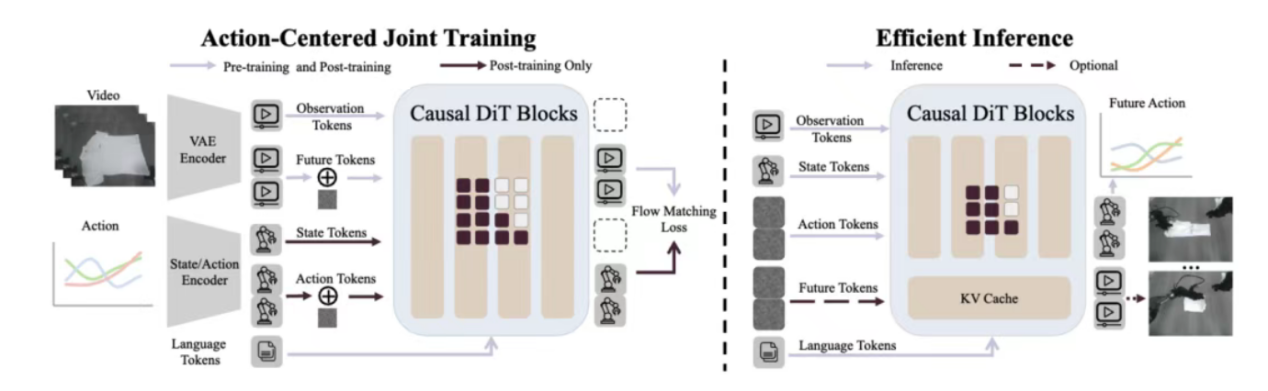
\includegraphics{images/image-0049.png}
\caption{GigaWorld-Policy 的动作中心联合训练与高效推理示意图}
\end{figure}

\hypertarget{ux4e8cux3c00.7vlaux6a21ux578b}{%
\subsubsection{（二）π0.7（VLA模型）}\label{ux4e8cux3c00.7vlaux6a21ux578b}}

π0.7涌现出组合泛化能力的关键在于，用多样化的prompt处理多样化的数据。过去VLA训练只喂一句清理冰箱，模型得到的信号是单一的。π0.7把prompt展开成四层：任务指令（清理厨房）+子任务指令（打开冰箱）+子目标图像（下一秒画面应该长什么样）+episode元数据（这条数据质量几分、有没有出错、速度多快）。

有了这些丰富的context，模型就能分得清训练数据里的好坏、快慢、对错。然后它就能吃下以前吃不了的数据。失败的rollouts，低质量的演示，其他机器人的片段，人类的egocentric视频，全都变成有用的信号。简而言之，π0.7加的那层prompt，就是让模型知道``这段数据是什么质量、用什么策略做的''。

\hypertarget{ux4e09ux9ad8ux5fb7abot-3dgsabot-physworldworld-modelux4f5cux4e3aux8badux7ec3ux73afux5883}{%
\subsubsection{（三）高德ABot-3DGS、ABot-PhysWorld（World Model作为训练环境）}\label{ux4e09ux9ad8ux5fb7abot-3dgsabot-physworldworld-modelux4f5cux4e3aux8badux7ec3ux73afux5883}}

先把数据转成机器能读懂的``多模态Clip''，比如骑车经过一个路口，高德记录下来的不只是一张图，而是一整套信息，包括路口长什么样（图像）、红绿灯在哪（空间位置）、现在是红灯还是绿灯（状态）、你是直行还是准备转弯（行为），甚至还包括周围有没有行人、车辆在动等，所有东西打包在一起就是一个Clip。ABot-3DGS利用这些Clip数据，重建3D真实场景；ABot-PhysWorld在这些场景中进行合乎物理定律（如滑动、倾倒、堆叠、流体变化）的动作推演。

对于ABot-PhysWorld的训练数据，高德精选300万条真实操作视频，用VLM+LLM双阶段标注，构建四层级物理语义结构，将数据拆解成机器人更易``消化''的结构化信息：

宏观层（意图）：自然语言描述整体任务目标，如``抓取并放置苹果''。

中观层（动作序列）：动词-名词短语序列，如``接近→抓握→提起→移动→释放''。

微观层（轨迹细节）：记录笛卡尔轨迹、相对运动、夹爪状态，如``末端沿Z轴下降5cm，夹爪闭合至20mm''。

场景层（物理关系）：描述接触、支撑、包含关系及任务结果，如``苹果与桌面接触，被夹爪稳固抓握，成功放置于袋中''。

这套标注流程不仅在告诉机器人``发生了什么''，更在解释``为什么发生''。

\hypertarget{ux53c2ux8003ux6587ux732e-172}{%
\subsection{参考文献}\label{ux53c2ux8003ux6587ux732e-172}}

\begin{itemize}
\tightlist
\item
  O'Neill, A., Rehman, A., Gupta, A., et al.~(2024). \href{https://arxiv.org/abs/2310.08864}{Open X-Embodiment: Robotic Learning Datasets and RT-X Models}. ICRA.
\item
  Walke, H., Black, K., Lee, A., et al.~(2023). \href{https://arxiv.org/abs/2308.12952}{BridgeData V2: A Dataset for Robot Learning at Scale}. arXiv:2308.12952.
\item
  Ye, A., Wang, B., Ni, C., et al.~(2026). \href{https://arxiv.org/abs/2603.17240}{GigaWorld-Policy: An Efficient Action-Centered World--Action Model}. arXiv:2603.17240.
\item
  Physical Intelligence, Ai, B., Amin, A., Aniceto, R., et al.~(2026). \href{https://arxiv.org/abs/2604.15483}{\(\pi_{0.7}\): a Steerable Generalist Robotic Foundation Model with Emergent Capabilities}. arXiv:2604.15483.
\item
  Yang, Y., Zeng, S., Lin, T., et al.~(2026). \href{https://arxiv.org/abs/2602.11236}{ABot-M0: VLA Foundation Model for Robotic Manipulation with Action Manifold Learning}. arXiv:2602.11236.
\item
  AMAP CV Lab. (2026). \href{https://amap-cvlab.github.io/ABot-Manipulation/}{ABot-M0: VLA Foundation Model for Robotic Manipulation with Action Manifold Learning}.
\item
  量子位. (2026). \href{https://www.traeai.com/articles/e175141a-e8b5-4e06-a589-42bd432aa115}{高德发布全球首个面向AGI的全栈具身技术体系``ABot''：15项SOTA，构建持续进化的具身智能闭环}.
\end{itemize}

\clearpage

\hypertarget{ux7b56ux7565ux51fdux6570ux7684ux8badux7ec3ux65b9ux6cd5}{%
\section{策略函数的训练方法}\label{ux7b56ux7565ux51fdux6570ux7684ux8badux7ec3ux65b9ux6cd5}}

在具身智能中，运动控制策略函数（即``小脑''）的训练是关键。

\hypertarget{ux4e00ux57faux4e8eux7ecfux5178ux63a7ux5236ux7406ux8bba}{%
\subsection{一、基于经典控制理论}\label{ux4e00ux57faux4e8eux7ecfux5178ux63a7ux5236ux7406ux8bba}}

这是最传统的机器人控制方法。

\begin{itemize}
\tightlist
\item
  核心逻辑：基于机器人的精确动力学方程（如拉格朗日动力学），在未来有限的时间窗口内，通过求解一个带约束的凸优化或非线性优化问题，计算出当前的最佳电机力矩。
\item
  数学建模：
\end{itemize}

假设``大脑''给出了未来 \(N\) 步的参考状态轨迹 \(x_k^{ref}\)，MPC``小脑''需要在满足动力学约束和不等式约束（如电机最大扭矩 \(u_{max}\)、足端接触摩擦锥限制）的前提下，最小化跟踪误差和能量消耗：

\[
\min_{u_{0:N-1}}
\sum_{k=0}^{N-1}
\left(
\|x_k-x_k^{ref}\|_Q^2+\|u_k\|_R^2
\right)
+
\|x_N-x_N^{ref}\|_{Q_f}^2
\]

\[
\text{s.t.}\quad x_{k+1}=f(x_k,u_k)\quad \mathcjk{（\mathcjk{刚体动力学}）}
\]

\[
h(x_k,u_k)\le 0\quad \mathcjk{（\mathcjk{物理与防碰撞约束}）}
\]

\begin{itemize}
\tightlist
\item
  工作流：

  \begin{enumerate}
  \def\labelenumi{\arabic{enumi}.}
  \tightlist
  \item
    指令接收：接收大脑下发的粗糙目标，如``向前走 1 米''或具体的足端落点。
  \item
    运动学与动力学建模：系统实时更新雅可比矩阵（Jacobian）和惯性矩阵。
  \item
    实时优化求解：利用二次规划（QP）求解器或非线性求解器（如基于牛顿法的内点法），以极高的频率（如 500Hz）实时计算出上述优化问题的解 \(u_0^*\)。
  \item
    力矩下发：将计算出的第一个控制指令 \(u_0^*\) 转换为电流信号，驱动底层伺服电机，并在下一个控制周期滚动重复此过程。
  \end{enumerate}
\end{itemize}

\hypertarget{ux4e8cux6a21ux4effux5b66ux4e60}{%
\subsection{二、模仿学习}\label{ux4e8cux6a21ux4effux5b66ux4e60}}

对于机械臂抓取、灵巧手操作等依赖高维视觉输入且难以设计密集奖励函数（Dense Reward）的任务，模仿学习是目前训练``小脑''的最前沿路线。近年来，基于扩散策略（Diffusion Policy）和动作分块（Action Chunking，如 ACT）的方法占据了统治地位。

\begin{itemize}
\tightlist
\item
  核心逻辑：跳过奖励函数的试错，直接利用神经网络拟合人类专家遥操作（Teleoperation）产生的高质量演示数据。
\item
  数学建模（以 Diffusion Policy 为例）：
\end{itemize}

扩散模型不再输出单一的确定动作，而是将动作生成建模为从随机噪声中逐步去噪的过程。给定大脑的指令 \(g\) 和当前的视觉/本体观测 \(o_t\)，模型预测一段未来连续步的动作轨迹序列 \(\mathbf{a}_{t:t+H}\)。其核心是训练一个条件噪声预测网络 \(\epsilon_\theta\)，最小化去噪过程的均方误差：

\[
\begin{aligned}
\mathcal{L}
&=
\mathbb{E}_{\mathbf{a}^0\sim\mathcal{D},\epsilon\sim\mathcal{N}(0,I),k}
\left[
\left\|
\epsilon-\epsilon_\theta(\mathbf{a}^k,o_t,g,k)
\right\|_2^2
\right]
\end{aligned}
\]

其中 \(\mathbf{a}^0\) 是真实的专家动作序列，\(\mathbf{a}^k\) 是加了 \(k\) 步前向高斯噪声的动作，\(\epsilon\) 是实际添加的噪声。

计算的是真实噪声与网络预测噪声之间的均方误差（MSE）。

公式中各项含义如下：

\begin{itemize}
\tightlist
\item
  \(\mathcal{L}\)：整体的损失函数。
\item
  \(\mathbb{E}\)：期望符号，代表在训练时对下标中的变量进行随机采样，并计算均值。
\item
  \(\mathbf{a}^0\sim\mathcal{D}\)：从人类专家示教数据集 \(\mathcal{D}\) 中采样出的真实动作序列（Ground Truth）。上标 0 代表这是未受任何污染的原始干净动作。在动作分块（Action Chunking）架构下，它通常不是单个动作，而是一段未来序列，例如未来 16 步的关节力矩向量。
\item
  \(\epsilon\sim\mathcal{N}(0,I)\)：从标准正态分布中采样出的真实高斯噪声。
\item
  \(k\)：扩散过程的时间步（Diffusion Step），通常从 1 到 \(K\)（例如 \(K=100\)）中均匀随机采样。
\item
  \(\mathbf{a}^k\)：带噪动作序列。它是将真实动作 \(\mathbf{a}^0\) 加上第 \(k\) 步对应强度的噪声 \(\epsilon\) 后得到的结果。\(k\) 越大，\(\mathbf{a}^k\) 越接近纯噪声。
\item
  \(o_t,g\)：条件变量（Conditions）。\(o_t\) 是机器人当前时刻的物理观测，如相机图像、本体关节角度；\(g\) 是语言指令或全局任务目标。
\item
  \(\epsilon_\theta(\cdot)\)：需要训练的神经网络，通常是带有交叉注意力机制的 1D U-Net 或 Transformer。\(\theta\) 是网络权重。它的输入是带噪动作 \(\mathbf{a}^k\) 以及条件变量，输出是它猜测的当初加进 \(\mathbf{a}^k\) 里的噪声 \(\epsilon\)。
\item
  \(\|\cdot\|_2^2\)：L2 范数的平方，即要求网络预测的噪声与实际添加的噪声尽可能一致。
\end{itemize}

工作流：

\begin{enumerate}
\def\labelenumi{\arabic{enumi}.}
\tightlist
\item
  数据采集：操作员使用动捕设备或 VR 手柄，在真实环境或仿真环境中控制机器人完成特定任务，记录下 \((o_t,g_t,a_t)\) 的轨迹对。
\item
  噪声注入与模型训练：在训练阶段，对专家动作序列注入不同时间步的高斯噪声。利用基于 CNN 或 Transformer 的 U-Net 架构，以视觉特征和指令特征作为条件（Condition），训练模型预测注入的噪声。
\item
  闭环推理执行：在实际部署时，模型接收实时观测，从纯高斯噪声开始，经过多步迭代去噪（如 DDIM 采样），生成一条平滑的未来动作轨迹。执行该轨迹的前几步后，重新观测环境并生成新轨迹（Receding Horizon Control）。
\end{enumerate}

\hypertarget{ux4e09ux5f3aux5316ux5b66ux4e60}{%
\subsection{三、强化学习}\label{ux4e09ux5f3aux5316ux5b66ux4e60}}

模仿学习具有显著的局限性，具身智能不能只会模仿人类，而是要能在探索中自主学习。因而强化学习是目前具身智能领域的核心和前沿，尤其擅长处理非线性动力学和复杂的环境接触。

``小脑''的策略被定义为参数化的概率分布 \(\pi_\theta(a_t|s_t,g_t)\)，其中 \(s_t\) 是本体感受器状态（如关节位置、IMU 数据），\(g_t\) 是大脑下发的子目标（如目标速度、目标位姿），\(a_t\) 是底层控制指令。

以 SAC 为例，其优化的目标函数不仅最大化累计奖励，还最大化策略的熵 \(\mathcal{H}\)，以鼓励探索并提升鲁棒性：

\[
\begin{aligned}
J(\pi_\theta)
&=
\mathbb{E}_{\tau\sim\pi_\theta}
\left[
\sum_{t=0}^{T}
\gamma^t
\left(
r(s_t,a_t,g_t)+
\alpha\mathcal{H}(\pi_\theta(\cdot|s_t,g_t))
\right)
\right]
\end{aligned}
\]

工作流（Sim2Real 范式）：

\begin{enumerate}
\def\labelenumi{\arabic{enumi}.}
\tightlist
\item
  仿真环境构建：在 Isaac Gym 或 MuJoCo 等高精度物理仿真器中建立机器人的数字孪生。
\item
  域随机化（Domain Randomization）：为了跨越``仿真到现实''（Sim2Real）的鸿沟，在训练时对物理参数（质量、摩擦系数、电机延迟、传感器噪声等）进行大幅度的随机采样。
\item
  大规模并行训练：利用 GPU 并行运行成千上万个环境，通过 PPO/SAC 算法收集轨迹数据，更新 Actor 网络（即``小脑''策略）和 Critic 网络。
\item
  真机部署（zero-shot Transfer）：将训练好的 Actor 网络权重直接冻结并部署到真实机器人控制器上，根据实时状态和大脑指令输出动作。
\end{enumerate}

强化学习的难点在于，需要在环境中试错，真机训练成本极为高昂。一种方法是引入基于世界模型的强化学习。以VLAW为例：

\begin{enumerate}
\def\labelenumi{\arabic{enumi}.}
\tightlist
\item
  收集真实世界数据：让 VLA 策略在真实世界中执行，收集少量包含成功与失败的轨迹数据，并标注离散的成功/失败奖励。
\item
  后训练世界模型与奖励模型：将收集到的真实轨迹数据与原始的机器人操作数据集结合，共同训练并微调预训练的世界模型，以防止模型对少量数据过拟合并提升其在特定任务上的物理准确性。同时，使用首轮真实数据微调视觉-语言奖励模型（Qwen3-VL-4B-Instruct），以提高奖励评估的保守度与准确性。
\item
  生成带奖励标签的合成轨迹：在更新后的世界模型中运行 VLA 策略，闭环自回归地生成大量合成轨迹。随后，利用预设好概率阈值的奖励模型对这些虚拟轨迹进行过滤，保留判定为成功的样本。
\item
  后训练 VLA 策略：整合过滤后的成功真实轨迹与成功合成轨迹，给成功轨迹分配权重 1，失败轨迹分配权重 0，使用流匹配（Flow-matching）目标函数对 VLA 策略进行更新。
\item
  循环迭代：交替重复上述步骤，不断协同提升世界模型和 VLA 策略的性能。
\end{enumerate}

后续内容会介绍世界模型与具身智能的具体结合方式。

\hypertarget{ux53c2ux8003ux6587ux732e-173}{%
\subsection{参考文献}\label{ux53c2ux8003ux6587ux732e-173}}

\begin{itemize}
\tightlist
\item
  Chi, C., Feng, S., Du, Y., Xu, Z., Cousineau, E., Burchfiel, B., \& Song, S. (2023). \href{https://arxiv.org/abs/2303.04137}{Diffusion Policy: Visuomotor Policy Learning via Action Diffusion}. RSS.
\item
  Zhao, T. Z., Kumar, V., Levine, S., \& Finn, C. (2023). \href{https://arxiv.org/abs/2304.13705}{Learning Fine-Grained Bimanual Manipulation with Low-Cost Hardware}. RSS.
\end{itemize}

\clearpage

\hypertarget{vlaux6a21ux578b}{%
\section{VLA模型}\label{vlaux6a21ux578b}}

VLA（Vision-Language-Action，视觉-语言-动作）模型正在引发一场范式革命，它打破了传统机器人``感知-规划-控制''的模块化割裂设计，将多模态大模型的语义推理能力直接映射为物理世界的底层执行动作。

\hypertarget{ux4e00ux6838ux5fc3ux601dux60f3-20}{%
\subsection{一、核心思想}\label{ux4e00ux6838ux5fc3ux601dux60f3-20}}

VLA模型的核心思想是``端到端''（End-to-End）的多模态深度融合。它将预训练的视觉-语言模型（VLM）作为``大脑''，把机器人的动作输出转化为一种特殊的``语言''，从而让大模型能够直接指挥物理硬件。

视觉（Vision）：通过视觉编码器（如ViT、SigLIP）将输入图像（如RGB摄像机画面流）切分为Patch，并转化为视觉Token，赋予机器人理解空间关系、物理属性的能力。

语言（Language）：接收人类的自然语言指令，结合预训练大模型积累的庞大互联网知识，提供逻辑推理与``常识''。

动作（Action）：VLA将动作词表化，将连续的机器人物理控制参数（如机械臂的关节扭矩、末端执行器的坐标）离散化，作为一种特殊的Token融入大语言模型的词表中。

\hypertarget{ux4e8cux81eaux56deux5f52vlaux8303ux5f0f}{%
\subsection{二、自回归VLA范式}\label{ux4e8cux81eaux56deux5f52vlaux8303ux5f0f}}

\hypertarget{ux4e00ux57faux672cux539fux7406-2}{%
\subsubsection{（一）基本原理}\label{ux4e00ux57faux672cux539fux7406-2}}

假设在时间步 \(t\)，智能体接收到视觉观测序列 \(o_{\le t}\in\mathcal{O}\) 以及自然语言指令 \(l\in\mathcal{L}\)，模型的目标是输出最优动作 \(a_t\in\mathcal{A}\)。

在以 RT-2（Robotic Transformer 2）和 OpenVLA 为代表的自回归（Autoregressive）VLA 范式中，连续动作 \(a_t\) 会被离散化为一系列动作 Token \((z_1,z_2,\ldots,z_K)\)。例如，一个 7 自由度（7-DoF）的机械臂动作可以表示为空间位移、旋转和夹爪开合度。

模型的训练目标是最大化以观测和指令为条件的动作 Token 的对数似然（Log-Likelihood）：

\[
\begin{aligned}
\mathcal{J}(\theta)
&=
\mathbb{E}_{(o,l,a)\sim\mathcal{D}}
\left[
\sum_{k=1}^{K}
\log P_{\theta}(z_k\mid z_{<k}, o_{\le t}, l)
\right]
\end{aligned}
\]

其中，\(\theta\) 为神经网络的参数，\(\mathcal{D}\) 为包含人类专家示范和互联网图文的混合数据集。通过这种方式，动作预测被完全等价转化为了类似于 ChatGPT 生成文本的 Next-token Prediction 任务。

\hypertarget{ux4e8cux5de5ux4f5cux6d41-6}{%
\subsubsection{（二）工作流}\label{ux4e8cux5de5ux4f5cux6d41-6}}

\begin{enumerate}
\def\labelenumi{\arabic{enumi}.}
\item
  多模态输入处理（Multimodal Input Processing）：步骤 1.1，获取当前相机的 RGB 图像 \(o_t\)，通过视觉编码器（Vision Encoder）提取特征，并经过 Projector（投影层）对齐到语言模型的特征空间，生成视觉 Token 序列；步骤 1.2，接收用户指令 \(l\)，通过文本分词器生成语言 Token 序列。
\item
  特征拼接与跨模态注意力计算（Context Concatenation \& Cross-modal Attention）：步骤 2.1，将系统提示词、视觉 Token 和语言 Token 按序列拼接为 \texttt{{[}System\ Prompt,\ Image\ Tokens,\ Language\ Tokens{]}}；步骤 2.2，送入 Transformer Decoder 骨干网络，通过自注意力机制（Self-Attention）让指令语义与图像中的物理特征产生深度绑定（Grounding）。
\item
  自回归动作生成（Autoregressive Action Generation）：步骤 3.1，Transformer 结合上下文，逐个预测当前步骤的动作 Token。例如先预测代表 \(A_x\) 的 Token，再将 \(A_x\) 作为已知条件预测 \(A_y\)，依次类推，直到输出夹爪动作 Token。
\item
  反词表化与物理控制（Detokenization and Execution）：步骤 4.1，将生成的动作 Token 序列 \((z_1,\ldots,z_K)\) 映射回连续的物理数值，生成实际控制指令；步骤 4.2，将指令发送给机器人底层控制器（如 PID 控制器）驱动电机执行。
\end{enumerate}

\hypertarget{ux4e09ux4f18ux7f3aux70b9}{%
\subsubsection{（三）优缺点}\label{ux4e09ux4f18ux7f3aux70b9}}

自回归VLA直接复用LLM的架构，天然继承了互联网级数据的逻辑链条（Chain-of-Thought）和常识推理能力。泛化能力极强，但受限于自回归的生成速度，高频连续控制能力略显不足。

\hypertarget{ux4e09ux6269ux6563ux6d41ux5339ux914dvlaux8303ux5f0f}{%
\subsection{三、扩散/流匹配VLA范式}\label{ux4e09ux6269ux6563ux6d41ux5339ux914dvlaux8303ux5f0f}}

这一范式的核心动机是消除``动作词表化''带来的离散化误差。它不再将动作强行转化为语言词表中的 Token，而是使用生成式连续时间模型（Diffusion Models 或 Flow Matching）直接在连续空间中生成高维、高频的动作轨迹（Action Chunks）。代表性模型包括 Physical Intelligence 的 \(\pi_0\)（Pi-Zero）、ForceVLA 等。

扩散/流匹配 VLA 通常采用 \textbf{``VLM + 动作专家（Action Expert）''} 的解耦与重组架构：

\begin{enumerate}
\def\labelenumi{\arabic{enumi}.}
\item
  多模态条件编码器：继承预训练的视觉语言模型（如 PaliGemma、SigLIP 结合 LLM 骨干），负责将图像序列 \(o\) 和语言指令 \(l\) 处理为深度的上下文条件嵌入（Condition Embeddings）。
\item
  连续动作生成器（Action Expert）：通常是 Diffusion Transformer（DiT）或 U-Net，接收上述条件嵌入，并通过交叉注意力机制（Cross-Attention）或拼接自注意力机制，对纯噪声信号进行迭代去噪，最终输出连续的物理动作块 \(A_t=(a_t,a_{t+1},\ldots,a_{t+H-1})\)。
\end{enumerate}

以目前先进的最优传输流匹配（Optimal Transport Flow Matching，类似于 \(\pi_0\) 中的设计）为例。假设基础噪声分布为 \(x_0\sim p_0=\mathcal{N}(0,I)\)，真实动作轨迹分布为 \(x_1\sim p_1\)，多模态条件为 \(c=\mathrm{Encoder}(o,l)\)。模型构建一条连接噪声与真实动作的直线概率路径：

\[
x_t=(1-t)x_0+t x_1
\]

动作生成器 \(v_\theta\) 的目标是拟合真实的速度场（Velocity Field），其目标函数定义为：

\[
\begin{aligned}
\mathcal{L}_{\mathrm{FM}}(\theta)
&=
\mathbb{E}_{\substack{t\sim \mathcal{U}(0,1)\\ x_0\sim p_0,\ x_1\sim p_1}}
\left[
\left\|v_\theta(x_t,t,c)-(x_1-x_0)\right\|^2
\right]
\end{aligned}
\]

这里 \((x_1-x_0)\) 是真实路径的恒定梯度。相较于传统的 DDPM 扩散模型，流匹配的 ODE 轨迹更加平滑且笔直，能够在极少的推理步数（甚至几步内）生成高保真的连续动作信号。
工作流：

\begin{enumerate}
\def\labelenumi{\arabic{enumi}.}
\item
  特征提取：VLM 接收当前相机观测和语言 \(l\)，前向传播生成多模态条件向量 \(c\)。
\item
  噪声初始化：从标准正态分布中采样一段长度为 \(H\) 的纯噪声轨迹 \(x_0\sim\mathcal{N}(0,I)\)。
\item
  常微分方程求解（ODE Solving）：在时间步 \(t\in[0,1]\) 之间，动作生成器 \(v_\theta(x_t,t,c)\) 结合上下文 \(c\) 计算当前状态的梯度，并通过数值积分器（如 Euler 法或 Heun 法）逐步更新。
\item
  动作执行：将 ODE 终点作为预测的动作块。系统采用模型预测控制（MPC/Receding Horizon Control）策略，仅执行前几个动作，随后重新获取新的视觉观测，进入下一轮闭环推理。
  优缺点：动作输出不再是离散 Token，而是通过 Diffusion Model（扩散模型）或 Flow Matching 直接生成连续的动作轨迹，在处理需要极高精度和灵巧度（如折叠衣服、灵巧手操作）的任务时表现出显著优势，但在长程任务的因果关系保持上可能不如自回归。
\end{enumerate}

\hypertarget{ux56dbux7edfux4e00ux8868ux5f81ux4e0eux6f5cux5728ux52a8ux4f5cux8303ux5f0f}{%
\subsection{四、统一表征与潜在动作范式}\label{ux56dbux7edfux4e00ux8868ux5f81ux4e0eux6f5cux5728ux52a8ux4f5cux8303ux5f0f}}

不同机器人的硬件形态之间（乃至与人类第一视角之间）存在差异。为了让VLA模型不被限制于特定的硬件中，而是可以利用海量无动作标签的视频进行扩展（Scaling），我们引入``抓取右上方的物体''等与具体硬件无关的统一潜在动作，而不是``右臂上抬30厘米''这样的具体机械操作。

在具身智能架构分类中，它介于分层和端到端之间，因为模型间传递的信息是可微的，梯度可以（在某些设计下）从底层直接传导回高层，或者在同一个世界模型的潜空间内完成对齐。

\hypertarget{ux4e00ux6838ux5fc3ux67b6ux6784-7}{%
\subsubsection{（一）核心架构}\label{ux4e00ux6838ux5fc3ux67b6ux6784-7}}

该路线的核心架构仍可拆成两部分：多模态条件编码器继承预训练的 VLM，将图像序列 \(o\) 与语言指令 \(l\) 编码为上下文条件嵌入；连续动作生成器接收这些条件嵌入，生成统一潜在动作块 \(A_t=(a_t,a_{t+1},\ldots,a_{t+H-1})\)。区别在于，高层输出的并不一定是某个机器人专属的底层控制量，而是可跨形态共享的潜在动作表示。

\hypertarget{ux4e8cux8badux7ec3ux65b9ux6cd5-1}{%
\subsubsection{（二）训练方法}\label{ux4e8cux8badux7ec3ux65b9ux6cd5-1}}

\begin{enumerate}
\def\labelenumi{\arabic{enumi}.}
\tightlist
\item
  训练阶段一：潜在动作空间的无监督学习（Latent Action Learning）。这一阶段不需要任何底层物理控制信号（如关节扭矩），模型仅通过观看海量视频序列来学习。模型通常引入一个基于 VQ-VAE（向量量化变分自编码器）的逆动力学模型（Inverse Dynamics Model）：输入连续两帧视频图像 \((o_t,o_{t+1})\)，编码器提取两帧之间的视觉和物理状态变化，生成连续隐特征；向量量化模块将连续隐特征映射到离散密码本（Codebook）中，提取以任务为中心的潜在动作 \(z_t\)；前向动力学模型接收当前帧 \(o_t\) 和潜在动作 \(z_t\)，尝试重建下一帧图像 \(\hat{o}_{t+1}\)。
\end{enumerate}

损失函数由重建损失和密码本正则化损失组成：

\[
\begin{aligned}
\mathcal{L}_{\mathrm{VQ}}
&= \|o_{t+1}-\hat{o}_{t+1}\|^2
+\|\mathrm{sg}[\mathrm{Encoder}(o_t,o_{t+1})]-e_{z_t}\|^2
\\
&\quad+
\beta\|\mathrm{Encoder}(o_t,o_{t+1})-\mathrm{sg}[e_{z_t}]\|^2
\end{aligned}
\]

其中，\(e_{z_t}\) 为密码本中的嵌入向量，\(\mathrm{sg}[\cdot]\) 为停止梯度操作。

\begin{enumerate}
\def\labelenumi{\arabic{enumi}.}
\setcounter{enumi}{1}
\tightlist
\item
  训练阶段二：联合策略优化与具身对齐（Joint Policy Optimization）。在获得跨形态潜在动作空间后，开始正式训练 VLA 大模型，将语义与物理硬件绑定。首先利用阶段一训练好的 VQ-VAE 编码器，把带有语言指令的机器人视频数据转化为``指令-图像-潜在动作 \(z_t\)''的离散序列数据；然后用标准的 Next-token Prediction 目标训练 VLM 主干网络，使其在给定图像和文本上下文时输出正确的潜在动作分布 \(P_\theta(z_t\mid o_{\le t},l)\)；最后引入轻量级形态感知解码器（Embodiment-aware Decoder）或联合扩散模块，将 VLM 输出的潜在动作 \(z_t\) 与当前机器人的专属形态标识拼接，并使用少量包含真实底层动作标签的数据训练该解码器：
\end{enumerate}

\[
\begin{aligned}
\mathcal{L}_{\mathrm{Action}}
&=
\mathbb{E}\left[
-\log P_\phi(a_t\mid z_t,o_t,\text{embodiment\_id})
\right]
\end{aligned}
\]

其中，目前业界部分实践在高层运用自回归以适配成熟生态，底层运用扩散以降低延迟。

\hypertarget{ux53c2ux8003ux6587ux732e-174}{%
\subsection{参考文献}\label{ux53c2ux8003ux6587ux732e-174}}

\begin{itemize}
\tightlist
\item
  Brohan, A., Brown, N., Carbajal, J., et al.~(2023). \href{https://arxiv.org/abs/2307.15818}{RT-2: Vision-Language-Action Models Transfer Web Knowledge to Robotic Control}. arXiv:2307.15818.
\item
  Kim, M. J., Pertsch, K., Karamcheti, S., et al.~(2024). \href{https://arxiv.org/abs/2406.09246}{OpenVLA: An Open-Source Vision-Language-Action Model}. arXiv:2406.09246.
\item
  Black, K., Brown, N., Driess, D., et al.~(2024). \href{https://arxiv.org/abs/2410.24164}{π0: A Vision-Language-Action Flow Model for General Robot Control}. arXiv:2410.24164.
\end{itemize}

\clearpage

\hypertarget{ux5177ux8eabux667aux80fdux7684ux672aux6765ux5c55ux671b}{%
\section{具身智能的未来展望}\label{ux5177ux8eabux667aux80fdux7684ux672aux6765ux5c55ux671b}}

大语言模型诞生后，AI在数字世界快速发展；具身智能则意味着AI向物理世界的拓展。下面是对未来具身智能发展的一些展望。

\hypertarget{ux4e00ux5177ux8eabux667aux80fdux7684ux57faux672cux5f62ux6001ux5c55ux671b}{%
\subsection{一、具身智能的基本形态展望}\label{ux4e00ux5177ux8eabux667aux80fdux7684ux57faux672cux5f62ux6001ux5c55ux671b}}

未来，我们希望基于具身智能的机器人能在足够丰富、足够复杂的现实任务里，像人类一样完成工作。这里引入``物理图灵测试''的概念，即人类已经无法仅靠观察去判断完成工作的是人类还是机器人。进一步来说，具身智能未来将不是独立的机器，而可以通过API或其他更高级的方式被调用。

\hypertarget{ux4e8cux5177ux8eabux667aux80fdux7684ux4e0bux6e38ux5e94ux7528ux5c55ux671b}{%
\subsection{二、具身智能的下游应用展望}\label{ux4e8cux5177ux8eabux667aux80fdux7684ux4e0bux6e38ux5e94ux7528ux5c55ux671b}}

在日常生活层面，具身智能将承担家务、照护、陪伴和家庭维修等任务。它不只是会执行固定动作的家电，而是能理解家庭成员的真实需求，感知复杂环境中的物品、老人、儿童和宠物状态，并在安全边界内自主规划行动，例如整理房间、准备餐食、照看老人、处理突发情况等。

在服务业层面，具身智能将进入餐饮、酒店、物流、医疗护理、零售和公共服务等场景。未来的机器人不仅能完成送餐、清洁、搬运、导览等重复性工作，也能根据顾客的语言、表情和行为作出灵活回应，从而让服务更稳定、更低成本，也让人类员工从高强度、低创造性的劳动中解放出来。

在工业层面，具身智能将实现工业生产的无人化。未来人类以自然语言等形式描述的需求可交由大模型得到可执行的生产方案，而实体生产过程可以完全由机器人自主完成。机器人可以操控流水线上的机器、监控生产状态，并对紧急状况及时作出反应。

在农业层面，具身智能将推动农业从依赖经验和人工劳动，走向精准化、自动化和数据化。机器人可以完成播种、除草、施肥、采摘、病虫害识别、土壤监测和农作物分拣等任务，并根据天气、土壤、水分和作物生长状态实时调整策略，从而提高产量、减少浪费，也缓解农业劳动力不足的问题。

在科学研究层面，如对于生物学中的临床样本处理、肿瘤切片、动物实验、复杂组织培养，以及执行全新实验流程、故障排错等硬编码难以处理的场景，具身智能可以将科学家从繁重的实验中解放出来，使其进行创造性思考而不是反复重做实验，并实现更多实验的标准化和数据统一，让AI Scientist从``窄域工业化闭环''走向``通用科学家闭环''。

\hypertarget{ux4e09ux5177ux8eabux667aux80fdux63a8ux52a8ux81eaux8eab}{%
\subsection{三、具身智能推动自身}\label{ux4e09ux5177ux8eabux667aux80fdux63a8ux52a8ux81eaux8eab}}

有认知理论认为，真正的智能的形成需要依赖与环境的互动。具身智能将能在现实世界大规模执行任务的同时，收集视觉、语言、传感器信号、环境状态变化等数据。结合这些交互数据训练模型，特别是结合带有``干预动作-状态转移''的因果数据和互联网视频难以触及的长尾数据训练模型，能让模型更好地理解物理世界及其因果关系，让模型具备真正意义上完全达到乃至超过人类水平的通用智能。

此外，机器人还可以自主设计、优化和制造下一代机器人，实现``Robots for robots''，极大地加速迭代。未来或许还将有为更多环境、更多用途打造的机器人，如纳米机器人、太空探索机器人、深海作业机器人、灾害救援机器人、极端环境维修机器人等。它们将把AI的能力从屏幕和服务器扩展到真实世界，使智能系统不只是``思考''和``生成''，而是能够真正行动、制造、探索和改变环境。

\hypertarget{ux53c2ux8003ux6587ux732e-175}{%
\subsection{参考文献}\label{ux53c2ux8003ux6587ux732e-175}}

\begin{itemize}
\tightlist
\item
  Varela, F. J., Thompson, E., \& Rosch, E. (2017). \href{https://mitpress.mit.edu/9780262529365/the-embodied-mind/}{The Embodied Mind: Cognitive Science and Human Experience} (Revised ed.). MIT Press. (Original work published 1991).
\item
  Brooks, R. A. (1991). \href{https://doi.org/10.1016/0004-3702\%2891\%2990053-M}{Intelligence without representation}. \emph{Artificial Intelligence}, 47(1-3), 139-159.
\item
  Sequoia Capital. (2025). \href{https://www.youtube.com/watch?v=_2NijXqBESI}{The Physical Turing Test: Jim Fan on Nvidia's Roadmap for Embodied AI}. YouTube.
\item
  Zhu, Y., Fan, L., \& NVIDIA GEAR Team. (2025). \href{https://research.nvidia.com/publication/2025-03_nvidia-isaac-gr00t-n1-open-foundation-model-humanoid-robots}{NVIDIA Isaac GR00T N1: An Open Foundation Model for Humanoid Robots}. NVIDIA Research.
\item
  Google DeepMind. (2025). \href{https://deepmind.google/models/gemini-robotics/}{Gemini Robotics}.
\item
  Brohan, A., Brown, N., Carbajal, J., et al.~(2023). \href{https://arxiv.org/abs/2307.15818}{RT-2: Vision-Language-Action Models Transfer Web Knowledge to Robotic Control}. arXiv:2307.15818.
\item
  O'Neill, A., Rehman, A., Gupta, A., et al.~(2024). \href{https://arxiv.org/abs/2310.08864}{Open X-Embodiment: Robotic Learning Datasets and RT-X Models}. ICRA.
\item
  Black, K., Brown, N., Driess, D., et al.~(2024). \href{https://arxiv.org/abs/2410.24164}{π0: A Vision-Language-Action Flow Model for General Robot Control}. arXiv:2410.24164.
\item
  Bousmalis, K., Vezzani, G., Rao, D., et al.~(2023). \href{https://arxiv.org/abs/2306.11706}{RoboCat: A Self-Improving Generalist Agent for Robotic Manipulation}. arXiv:2306.11706.
\item
  Lu, C., Lu, C., Lange, R. T., Foerster, J., Clune, J., \& Ha, D. (2024). \href{https://arxiv.org/abs/2408.06292}{The AI Scientist: Towards Fully Automated Open-Ended Scientific Discovery}. arXiv:2408.06292.
\end{itemize}

\clearpage
